

\begin{definition}[Aperiodicity]
A random walk defined by a Markov chain having state space $S$ and state transition matrix $P$ ,is said to be aperiodic if there exists self-transition in the chain such that
\begin{align}
    p^n_{ii}>0 \quad \text{for} \quad i \in S,n \in Z^+
\end{align}
\end{definition}

\begin{definition}[Irreducibility]
A random walk defined by a Markov chain having state space $S$ and state transition matrix $P$ ,is said to be irreducible if all states communicate with each other such that
\begin{align}
    p^n_{ij}>0 \quad \text{for} \quad i,j \in S,n \in Z^+
\end{align}
\end{definition}

\begin{definition}[Positive and Null Recuurancy]
A random walk defined by a Markov chain having state space $S$ ,is said to be positive recurrent if the excepted time to return to state $i$ $\forall$ $i \in S$ is finite such that
\begin{align}
    E(\tau_{ii}) < \infty
\end{align}

and,is said to be null recurrent if the excepted time to return to state $i$ $\forall$ $i \in S$ is infinite such that
\begin{align}
    E(\tau_{ii}) = \infty
\end{align}
\end{definition}

Let us define a Markov Chain for the given simple symmetric random walk with states $\cbrak{i-1,i,i+1}$ .

\begin{figure}[!ht]
\centering
\begin{tikzpicture}
    % Setup the style for the states
        \tikzset{node style/.style={state, 
                                    minimum width=0.2cm,
                                    line width=0.75mm,
                                    fill=gray!20!white}}
        % Draw the states
        \node[node style] at (0,0)      (state_i)   {i};     
        \node[node style] at (2,0)      (state_i+1) {i+1};      
        \node[node style] at (-2,0)     (state_i-1) {i-1};  
        %\node[node style] at (4, 0)     (state_i+2) {i+2}; 
        %\node[node style] at (-4, 0)    (state_i-2) {i-2};
        \draw[line width =0.5mm,loosely dotted] (2.5,0) -- (4,0);
        \draw[line width =0.5mm,loosely dotted] (-2.5,0) -- (-4,0);
        % Connect the states with arrows
        \draw[every loop,
              auto=right,
              line width=0.7mm,
              >=latex,
              draw=orange,
              fill=orange]
        (state_i) edge[bend right = 20] node{$\frac{1}{2}$} (state_i+1)
        (state_i+1) edge[bend right = 20] node{$\frac{1}{2}$} (state_i)
        (state_i) edge[bend right = 20] node{$\frac{1}{2}$}  (state_i-1)
        (state_i-1) edge[bend right = 20] node{$\frac{1}{2}$}  (state_i);
\end{tikzpicture}
\caption{\textbf{Markov chain diagram}}
\label{markov/8/texfig}
\end{figure}

State transition matrix $P$ can be defined as:
\begin{align}
\label{markov/8/cs2015-291}
    P=\begin{blockarray}{cccc}
& i-1 & i & i+1 \\
\begin{block}{c[ccc]}
  i-1 & 0 & \frac{1}{2}  & \frac{1}{4}  \\
  i & \frac{1}{2} & 0 & \frac{1}{2} \\
  i+1 & \frac{1}{4} & \frac{1}{2} & 0 \\
\end{block}
\end{blockarray}
\end{align}

\begin{enumerate}
    \item From State Transition Matrix $P$,
      \begin{align}
        p_{mm} = 0
    \end{align}
    where
    \begin{align}
        m=\{i-1,i,i+1\} 
    \end{align}
    
    $\because$ There is no self-transition in the chain.
    
    $\therefore$ Random Walk is not aperiodic.

    \item From State Transition Matrix $P$,
    \begin{align}
        p_{mn} > 0  
    \end{align}
    where
    \begin{align}
        m,n=\{i-1,i,i+1\} 
    \end{align}
     
    $\because$ All states communicate with each other .

    $\therefore$ Random Walk is irreducible.

    \item Let $p=\frac{1}{2}$ be the probability to move from state $i$ to state $i+1$ and $q=\frac{1}{2}$ be the probability to move from state $i$ to state $i-1$ .

    Then,the excepted time of getting back to $i$ $\forall$ $i$ is given by 
    \begin{align}
       E(\tau_{ii}) &= \frac{1}{|p-q|} \\
       &=\frac{1}{0} \\
       &= \infty
    \end{align}

    $\therefore$ Random Walk is null recurrent .

\end{enumerate}

Hence, \boxed{Options \quad (2),(3)} are true .


\begin{figure}[!ht]
\centering
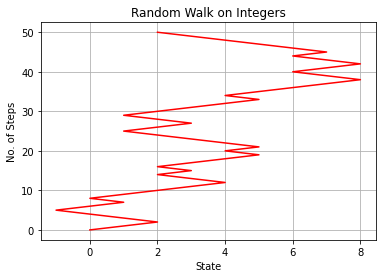
\includegraphics[width=\columnwidth]{markov/solutions/8/Figure18.png}
\caption{Random Walk on Integers}
\label{markov/8/Random Walk}	
\end{figure}




